\documentclass[12pt]{article}

\usepackage{natbib}
\usepackage{apalike}
\usepackage[hypertexnames=false,colorlinks=true,breaklinks]{hyperref}
\usepackage{amsthm}
\usepackage{amsmath}
\usepackage{amssymb}
\usepackage{graphicx}
\usepackage[margin=2.0cm]{geometry}
\usepackage{xcolor}
\usepackage{graphicx}
\usepackage{siunitx}
\sisetup{output-exponent-marker=\ensuremath{\mathrm{e}}}
\usepackage{tikz}
\usepackage{subcaption}
% \usepackage{endfloat}

\usetikzlibrary{bayesnet}

\newtheorem{lemma}{Lemma}
\newtheorem{theorem}{Theorem}

\title{Inference in Linear Dynamical Systems}
\author{Joaquin Rapela\thanks{j.rapela@ucl.ac.uk}}

\begin{document}

\maketitle

\section{Linear dynamical systems (LDS) model}
\label{sec:ldsModel}

\begin{alignat*}{2}
    \mathbf{x}_{n+1}&=A_n\mathbf{x}_n+\mathbf{w}_n&\quad&\text{with }\mathbf{w}_n\sim N(0,Q_n)\\
    \mathbf{y}_n&=B_n\mathbf{x}_n+\mathbf{v}_n&&\text{with }\mathbf{v}_n\sim N(0,R_n)\\
    \mathbf{x}_0&\sim N(\mathbf{m}_0,V_0)&&
\end{alignat*}

\begin{figure}[h]
\begin{center}
    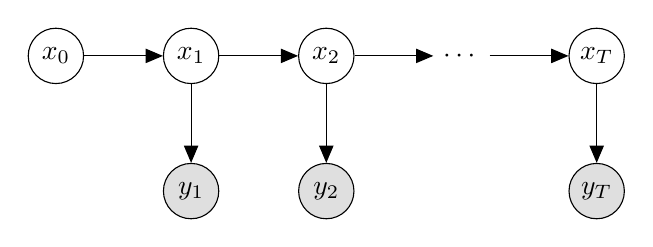
\begin{tikzpicture}[node distance=2.5cm and 1.8cm]

  % Nodes for hidden states
  \node[latent]              (x0) {$x_0$};
  \node[latent, right=of x0] (x1) {$x_1$};
  \node[latent, right=of x1] (x2) {$x_2$};
  \node[latent, right=of x2, draw=none] (xD) {$\cdots$};
  \node[latent, right=of xD] (xT) {$x_T$};

  % Nodes for observations
  \node[obs, below=of x1] (y1) {$y_1$};
  \node[obs, below=of x2] (y2) {$y_2$};
  \node[obs, below=of xT] (yT) {$y_T$};

  % Edges between hidden states
  \edge {x0} {x1};
  \edge {x1} {x2};
  \edge {x2} {xD};
  \edge {xD} {xT};

  % Emission edges
  \edge {x1} {y1};
  \edge {x2} {y2};
  \edge {xT} {yT};

\end{tikzpicture}

    \label{fig:ldsGraphicalModel}
    \caption{Graphical models for the linear dynamical system}
\end{center}
\end{figure}

\section{Inference Problems}
\label{sec:inferenceProblems}

\begin{description}
    \item[Prediction]
        \begin{align}
            P(\mathbf{x}_n|\mathbf{y}_1,\ldots,\mathbf{y}_{n-1})=N(\mathbf{x}_n|\mathbf{x}_{n|n-1},P_{n|n-1})\label{eq:prediction}
        \end{align}
    \item[Filtering]
        \begin{align}
            P(\mathbf{x}_n|\mathbf{y}_1,\ldots,\mathbf{y}_{n})=N(\mathbf{x}_n|\mathbf{x}_{n|n},P_{n|n})\label{eq:filtering}
        \end{align}
    \item[Smoothing]
        \begin{align}
            P(\mathbf{x}_n|\mathbf{y}_1,\ldots,\mathbf{y}_{N})=N(\mathbf{x}_n|\mathbf{x}_{n|N},P_{n|N})\label{eq:smoothing}
        \end{align}
    \item[Forecasting]
        \begin{align}
            P(\mathbf{x}_{n+h}|\mathbf{y}_1,\ldots,\mathbf{y}_{n})=N(\mathbf{x}_n|\mathbf{x}_{n+h|n},P_{n+h|n})\label{eq:forecasting}
        \end{align}
\end{description}

\section{Kalman Filter}

The Kalman filter algorithm addresses the prediction (Eq.~\ref{eq:prediction})
and filtering (Eq.~\ref{eq:filtering}) inference problems.
%
It is an iterative algorithm, which alternates between computing the mean and
covariance of the prediction distribution and computing the mean and covariance
of the filtering distribution.

Inference of predicted and filtered means and covariances proceeds in a forward
fashion, inferring the prediction and filtering distributions from the first to
the last state, as shown in the next figure.

\begin{figure}[h]
\begin{center}
    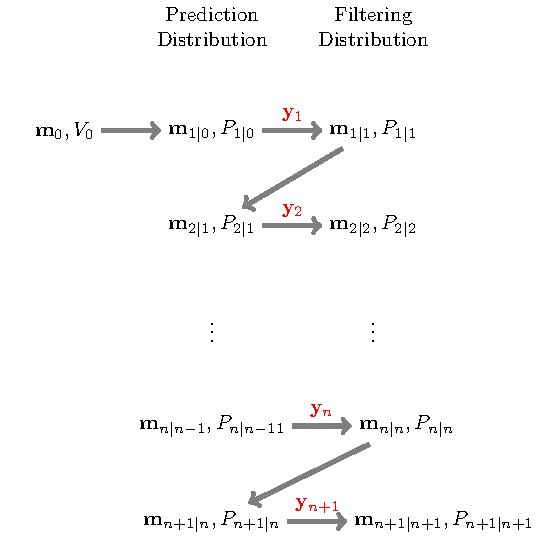
\includegraphics[width=5in]{figures/kfAlternations.pdf}
    \caption{Order of calculation of the prediction and filtering distributions
    in the Kalman filtering algorithm.}
    \label{fig:kfAlternations.}
\end{center}
\end{figure}

\section{Derivation of Kalman filter equations}

\begin{theorem}
	\label{thm:kalmanFilterEqs}

    Given the linear dynamical systems model given in
    Section~\ref{sec:ldsModel} then the means and covariances of the prediction
    (Eq.~\ref{eq:prediction}) and filtering (Eq.~\ref{eq:filtering})
    distributions are calculated iteratively as follows:

    \begin{alignat}{2}
        \mathbf{x}_{0|0}&=\mathbf{m}_0&&\text{init filtered mean}\label{eq:x0G0}\\
        P_{0|0}&=V_0&&\text{init filtered covariance}\label{eq:P0G0}\\
        \mathbf{x}_{n|n-1}&=A_{n-1}\mathbf{x}_{n-1|n-1}&&\text{prediction mean}\label{eq:xtGtm1}\\
        P_{n|n-1}&=A_{n-1}P_{n-1|n-1}A_{n-1}^\intercal+Q_{n-1}&&\text{prediction covariance}\label{eq:PtGtm1}\\
        \hat{\mathbf{y}}_{n|n-1}&\triangleq E\{\mathbf{y}_n|\mathbf{y}_1,\ldots,\mathbf{y}_{n-1}\}=B_n\mathbf{x}_{n|n-1}&&\text{predicted observation}\label{eq:ytGtm1}\\
        \mathbf{z}_n&\triangleq\mathbf{y}_n-\hat{\mathbf{y}}_{n|n-1}&&\text{residual}\nonumber\\
        S_n&\triangleq \text{Cov}\{\mathbf{z}_n|\mathbf{y}_1,\ldots,\mathbf{y}_{n-1}\}=B_nP_{n|n-1}B_n^\intercal+R_n\quad&&\text{residual covariance}\label{eq:St}\\
        \mathbf{K}_n&=P_{n|n-1}B_n^\intercal S_n^{-1}&&\text{Kalman gain}\label{eq:Kt}\\
        \mathbf{x}_{n|n}&=\mathbf{x}_{n|n-1}+K_n\mathbf{z}_n&&\text{filtering mean}\label{eq:xtGt}\\
        \mathbf{P}_{n|n}&=(I-K_nB_n)P_{n|n-1}&&\text{filtering covariance}\label{eq:PtGt}
    \end{alignat}

\end{theorem}

The following proof adds details to that given in Section 4.3.1 of
\citet{durbinAndKoopman12}.

\begin{proof}
    Call $Y_n=\{\mathbf{y}_1,\ldots,\mathbf{y}_n\}$, then

    \begin{align}
        \mathbf{x}_{n|n-1}&=E\{\mathbf{x}_n|Y_{n-1}\}=E\{A_{n-1}\mathbf{x}_{n-1}+\mathbf{w}_{n-1}|Y_{n-1}\}\nonumber\\
                          &=A_{n-1}E\{\mathbf{x}_{n-1}|Y_{n-1}\}+E\{\mathbf{w}_{n-1}|Y_{n-1}\}\nonumber\\
                          &=A_{n-1}\mathbf{x}_{n-1|n-1}+E\{\mathbf{w}_{n-1}\}\footnotemark[1]=A_{n-1}\mathbf{x}_{n-1|n-1}\nonumber
    \end{align}
    \footnotetext[1]{$\mathbf{w}_{n-1}$ is independent of $Y_{n-1}$.}
	This proves Eq.~\ref{eq:xtGtm1}.

    \begin{align}
        \mathbf{P}_{n|n-1}&=\text{Cov}\{\mathbf{x}_n|Y_{n-1}\}=E\{(\mathbf{x}_n-\mathbf{x}_{n|n-1})(\mathbf{x}_n-\mathbf{x}_{n|n-1})^\intercal|Y_{n-1}\}\nonumber\\
                          &=E\{\left(A_{n-1}\mathbf{x}_{n-1}+w_{n-1}-A_{n-1}\mathbf{x}_{n-1|n-1}\right)\left(A_{n-1}\mathbf{x}_{n-1}+w_{n-1}-A_{n-1}\mathbf{x}_{n-1|n-1}\right)^\intercal|Y_{n-1}\}\nonumber\\
                          &=E\{\left(A_{n-1}(\mathbf{x}_{n-1}-\mathbf{x}_{n-1|n-1})+w_{n-1}\right)\left(A_{n-1}(\mathbf{x}_{n-1}-\mathbf{x}_{n-1|n-1})+w_{n-1}\right)^\intercal|Y_{n-1}\}\nonumber\\
                          &=A_{n-1}E\{(\mathbf{x}_{n-1}-\mathbf{x}_{n-1|n-1})(\mathbf{x}_{n-1}-\mathbf{x}_{n-1|n-1})^\intercal|Y_{n-1}\}A_{n-1}^\intercal+\nonumber\\
                          &\qquad E\{w_{n-1}(\mathbf{x}_{n-1}-\mathbf{x}_{n-1|n-1})^\intercal|Y_{n-1}\}A_{n-1}^\intercal+\nonumber\\
                          &\qquad A_{n-1}E\{(\mathbf{x}_{n-1}-\mathbf{x}_{n-1|n-1})w_{n-1}^\intercal|Y_{n-1}\}+\nonumber\\
                          &\qquad E\{w_{n-1}w_{n-1}^\intercal|Y_{n-1}\}\nonumber\\
                          &=A_{n-1}E\{(\mathbf{x}_{n-1}-\mathbf{x}_{n-1|n-1})(\mathbf{x}_{n-1}-\mathbf{x}_{n-1|n-1})^\intercal|Y_{n-1}\}A_{n-1}^\intercal+\nonumber\\
                          &\qquad E\{w_{n-1}|Y_{n-1}\}E\{(\mathbf{x}_{n-1}-\mathbf{x}_{n-1|n-1})^\intercal|Y_{n-1}\}A_{n-1}^\intercal\footnotemark[2]+\nonumber\\
                          &\qquad A_{n-1}E\{(\mathbf{x}_{n-1}-\mathbf{x}_{n-1|n-1})|Y_{n-1}\}E\{w_{n-1}^\intercal|Y_{n-1}\}+\nonumber\\
                          &\qquad E\{w_{n-1}w_{n-1}^\intercal\}\nonumber\\
                          &=A_{n-1}P_{n-1|n-1}A_{n-1}^\intercal+Q_{n-1}\footnotemark[3]\nonumber
    \end{align}
    \footnotetext[2]{$\mathbf{w}_{n-1}$ is independent of $x_{n-1}$ given $Y_{n-1}$.}
    \footnotetext[3]{$E\{\mathbf{x}_{n-1}-\mathbf{x}_{n-1|n-1}|Y_{n-1}\}=E\{\mathbf{x}_{n-1}|Y_{n-1}\}-\mathbf{x}_{n-1|n-1}=\mathbf{x}_{n-1|n-1}-\mathbf{x}_{n-1|n-1}=0$.}
	This proves Eq.~\ref{eq:PtGtm1}.

    \begin{align}
        \hat{\mathbf{y}}_{n|n-1}&=E\{\mathbf{y}_n|Y_{n-1}\}=E\{B_n\mathbf{x}_n+\mathbf{v}_n|Y_{n-1}\}=B_nE\{\mathbf{x}_n|Y_{n-1}\}+E\{\mathbf{v}_n|Y_{n-1}\}\nonumber\\
                                &=B_n\mathbf{x}_{n|n-1}+E\{\mathbf{v}_n\}=B_n\mathbf{x}_{n|n-1}\nonumber
    \end{align}
	This proves Eq.~\ref{eq:ytGtm1}.

    Because

    \begin{align}
        \mathbf{z}_n&=\mathbf{y}_n-\hat{\mathbf{y}}_{n|n-1}=B_n\mathbf{x}_n+\mathbf{v}_n-B_n\mathbf{x}_{n|n-1}=B_n(\mathbf{x}_n-\mathbf{x}_{n|n-1})+\mathbf{v}_n\label{eq:ztProof}
    \end{align}

    \noindent $Y_{n-1}$ and $\mathbf{z}_n$ are fixed if and only if $Y_n$ is
    fixed\footnotemark[4]. Then

    \footnotetext[4]{If we now $Y_{n-1}$ and $\mathbf{z}_n$, then we know
    $\hat{\mathbf{y}}_{n|n-1}$ and $\mathbf{z}_n$, then (by the first equality
    in Eq.~\ref{eq:ztProof}) we know $\mathbf{y}_n$, thus we know $Y_n$. Also, if we
    know $Y_n$, we know $\hat{\mathbf{y}}_{n|n-1}$ and $\mathbf{y}_n$ and (by
    the first equality in Eq.~\ref{eq:ztProof}) we know $\mathbf{z}_n$.}.

    \begin{align}
        \mathbf{x}_{n|n}&=E\{\mathbf{x}_n|Y_n\}=E\{\mathbf{x}_n|Y_{n-1},\mathbf{z}_n\}\footnotemark[5]\nonumber\\
                        &=E\{\mathbf{x}_n|Y_{n-1}\}+\text{Cov}\left(\mathbf{x}_n,\mathbf{z}_n|Y_{n-1}\right)\text{Cov}\left(\mathbf{z}_n|Y_{n-1}\right)^{-1}\mathbf{z}_n\footnotemark[6]\label{eq:xtGtTmp}\\
        \text{Cov}\left(\mathbf{x}_n,\mathbf{z}_n|Y_{n-1}\right)&=\text{Cov}\left(\mathbf{x}_n,B_n(\mathbf{x}_n-\mathbf{x}_{n|n-1})+\mathbf{v}_n|Y_{n-1}\right)\nonumber\\
                                                                &=E\{(\mathbf{x}_n-\mathbf{x}_{n|n-1})(B_n(\mathbf{x}_n-\mathbf{x}_{n|n-1})+\mathbf{v}_n)^\intercal|Y_{n-1}\}\nonumber\\
                                                                &=E\{(\mathbf{x}_n-\mathbf{x}_{n|n-1})(\mathbf{x}_n-\mathbf{x}_{n|n-1})^\intercal|Y_{n-1}\}B_n^\intercal\nonumber\\
                                                                &\qquad +E\{(\mathbf{x}_n-\mathbf{x}_{n|n-1})\mathbf{v}_n^\intercal|Y_{n-1}\}\nonumber\\
                                                                &=P_{n|n-1}B_n^\intercal\footnotemark[7]\label{eq:covXZ}\\
        S_n=\text{Cov}\left(\mathbf{z}_n|Y_{n-1}\right)&=E\{\mathbf{z}_n\mathbf{z}_n^\intercal|Y_{n-1}\}\nonumber\\
                                                       &=E\{\left(B_n(\mathbf{x}_n-\mathbf{x}_{n|n-1})+\mathbf{v}_n\right)\left(B_n(\mathbf{x}_n-\mathbf{x}_{n|n-1})+\mathbf{v}_n\right)^\intercal|Y_{n-1}\}\footnotemark[8]\nonumber\\
                                                       &=B_nE\{\left(\mathbf{x}_n-\mathbf{x}_{n|n-1}\right)\left(\mathbf{x}_n-\mathbf{x}_{n|n-1}\right)^\intercal|Y_{n-1}\}B_n^\intercal+B_nE\{\left(\mathbf{x}_n-\mathbf{x}_{n|n-1}\right)\mathbf{v}_n^\intercal|Y_{n-1}\}\nonumber\\
                                                       &\qquad +E\{\mathbf{v}_n\left(\mathbf{x}_n-\mathbf{x}_{n|n-1}\right)^\intercal\}B_n^\intercal+E\{\mathbf{v}_n\mathbf{v_n}^\intercal|Y_{n-1}\}\nonumber\\
                                                       &=B_nE\{\left(\mathbf{x}_n-\mathbf{x}_{n|n-1}\right)\left(\mathbf{x}_n-\mathbf{x}_{n|n-1}\right)^\intercal|Y_{n-1}\}B_n^\intercal+\nonumber\\
                                                       &\qquad +E\{\mathbf{v}_n\mathbf{v_n}^\intercal\}\footnotemark[7]\footnotemark[9]\nonumber\\
                                                       &=B_nP_{n|n-1}B_n^\intercal+R_n\label{eq:covZ}
    \end{align}
    \footnotetext[5]{The validity of the last equality follow from measure theory arguments (that I don't know).}
    \footnotetext[6]{Refer to Eq.~\ref{eq:conditionalMean} in Lemma~\ref{lemma:conditionalGaussians}.}
    \footnotetext[7]{$E\{(\mathbf{x}_n-\mathbf{x}_{n|n-1})\mathbf{v}_n^\intercal|Y_{n-1}\}=E\{\mathbf{x}_n-\mathbf{x}_{n|n-1}|Y_{n-1}\}E\{\mathbf{v}_n^\intercal|Y_{n-1}\}=(E\{\mathbf{x}_n|Y_{n-1}\}-\mathbf{x}_{n|n-1})E\{\mathbf{v}_n^\intercal|Y_{n-1}\}=(\mathbf{x}_{n|n-1}-\mathbf{x}_{n|n-1})E\{\mathbf{v}_n^\intercal|Y_{n-1}\}=0$
    because $\mathbf{x}_n$ is independent of $\mathbf{v}_n$ given $Y_{n-1}$.}
    \footnotetext[8]{Eq.~\ref{eq:ztProof}.}
    \footnotetext[9]{$\mathbf{v}_n$ is independent from $Y_{n-1}$.}

	This proves Eq.~\ref{eq:St}.

    Combining Eqs.~\ref{eq:xtGtTmp}, \ref{eq:covXZ} and~\ref{eq:covZ} we obtain

    \begin{align}
        \mathbf{x}_{n|n}&=\mathbf{x}_{n|n-1}+P_{n|n-1}B_n^\intercal
        S_n^{-1}\mathbf{z}_n\nonumber\\
                        &=\mathbf{x}_{n|n-1}+K_n\mathbf{z}_n\quad\text{with } K_n=P_{n|n-1}B_n^\intercal S_n^{-1}\nonumber\\
        P_{n|n}&=\text{Cov}(\mathbf{x}_n|Y_n)=\text{Cov}(\mathbf{x}_n|Y_{n-1},\mathbf{z}_n)=P_{n|n-1}-P_{n|n-1}B_n^\intercal
        S_n^{-1}B_nP_{n|n-1}\footnotemark[10]\nonumber\\
               &=\left(I-P_{n|n-1}B_n^\intercal S_n^{-1}B_n\right)P_{n|n-1}=\left(I-K_nB_n\right)P_{n|n-1}\nonumber
    \end{align}
    \footnotetext[10]{Refer to Eq.~\ref{eq:conditionalCov} in Lemma~\ref{lemma:conditionalGaussians} with $\mathbf{x}=\mathbf{x}_n|Y_{n-1}$ and $\mathbf{y}=\mathbf{z}_n|Y_{n-1}$ giving

		\begin{align*}
			\Sigma_{x|y}&=\Sigma_{\mathbf{x}_n|\mathbf{z}_n,Y_{n-1}}=\Sigma_{\mathbf{x}_n|Y_n}=P_{n|n}\\
			\Sigma_{xx}&=\Sigma_{\mathbf{x}_n|Y_{n-1}}=P_{n|n-1}\\
			\Sigma_{xy}&=\Sigma_{\mathbf{x}_n\mathbf{z}_n|Y_{n-1}}=\text{Cov}(\mathbf{x}_n,\mathbf{z}_n|Y_{n-1})=P_{n|n-1}B_n^\intercal\\
			\Sigma_{yy}&=\Sigma_{\mathbf{z}_n\mathbf{z}_n|Y_{n-1}}=\text{Cov}(\mathbf{z}_n|Y_{n-1})=S_n\\
                        &\text{thus}\\
            P_{n|n}&=P_{n|n-1}-P_{n|n-1}B_n^\intercal S_n^{-1}B_nP_{n|n-1}
		\end{align*}
    }
	This proves Eqs.~\ref{eq:Kt}, \ref{eq:xtGt} and~\ref{eq:PtGt}.

	Using Eqs.~\ref{eq:x0G0} and~\ref{eq:P0G0} in Eqs.~\ref{eq:xtGtm1} and~\ref{eq:PtGtm1} we obtain

    \begin{align*}
        \mathbf{x}_{1|0}&=A_0\mathbf{x}_{0|0}=A_0\mathbf{m}_0\\
        \mathbf{P}_{1|0}&=A_0P_{0|0}A_0^\intercal+Q_0=A_0V_0A_0^\intercal+Q_0
    \end{align*}

	If Eqs.~\ref{eq:x0G0} and~\ref{eq:P0G0} are correct, then the density of $\mathbf{x}_1$ should be $p(\mathbf{x}_1)=\mathcal{N}(\mathbf{x}_1|\mathbf{x}_{1|0},P_{1|0})$. We now calculate this density using the linear dynamical system model in Theorem~\ref{thm:kalmanFilterEqs}.

    \begin{align}
		p(\mathbf{x}_1)&=\int p(\mathbf{x}_1,\mathbf{x}_0)d\mathbf{x}_0=\int p(\mathbf{x}_1|\mathbf{x}_0)p(\mathbf{x}_0)d\mathbf{x}_0=\int\mathcal{N}(\mathbf{x}_1|A_0\mathbf{x}_0,Q_0)\mathcal{N}(\mathbf{x}_0|\mathbf{m}_0,V_0)d\mathbf{x}_0\nonumber\\
                       &=\mathcal{N}(\mathbf{x}_1|A_0\mathbf{m}_0,A_0V_0A_0^\intercal+Q_0)\footnotemark[11]=\mathcal{N}(\mathbf{x}_1|\mathbf{x}_{1|0},\mathbf{P}_{1|0})\nonumber
    \end{align}
    \footnotetext[11]{Lemma~\ref{lemma:linearModelGaussianLatents}.}
	This proves Eqs.~\ref{eq:x0G0} and~\ref{eq:P0G0}.

\end{proof}

\pagebreak

\begin{lemma}

    Let $\mathbf{x}$ and $\mathbf{y}$ be jointly Gaussian distributed random
    vectors with

    \begin{align*}
        E\left\{\left[\begin{array}{c}
                          \mathbf{x}\\
                          \mathbf{y}
                      \end{array}\right]\right\}&=\left[\begin{array}{c}
                                                           \boldsymbol{\mu}_x\\
                                                           \boldsymbol{\mu}_y
                                                       \end{array}\right]\\
        \text{Cov}\left\{\left[\begin{array}{c}
                                   \mathbf{x}\\
                                   \mathbf{y}
                               \end{array}\right]\right\}&=\left[\begin{array}{cc}
                                                                     \Sigma_{xx} & \Sigma_{xy} \\
                                                                     \Sigma_{yx} & \Sigma_{yy} \\
                                                                  \end{array}\right]
    \end{align*}

    \noindent where $\Sigma_{yy}$ is assumed to be non-singular.
    %
    Then the conditional distribution of $\mathbf{x}$ given $\mathbf{y}$ is
    Gaussian with mean vector

    \begin{align}
        \text{E}\{\mathbf{x}|\mathbf{y}\}=\boldsymbol{\mu}_x+\Sigma_{xy}\Sigma_{yy}^{-1}(\mathbf{y}-\boldsymbol{\mu}_y)\label{eq:conditionalMean}
    \end{align}

    \noindent and covariance matrix

    \begin{align}
        \text{Cov}\{\mathbf{x}|\mathbf{y}\}=\Sigma_{xx}-\Sigma_{xy}\Sigma_{yy}^{-1}\Sigma_{yx}\label{eq:conditionalCov}
    \end{align}

    \label{lemma:conditionalGaussians}

\end{lemma}

\begin{proof}
    Let

    \begin{align}
        \mathbf{z}=\mathbf{x}-\Sigma_{xy}\Sigma_{yy}^{-1}(\mathbf{y}-\boldsymbol{\mu}_y)\label{eq:z}
    \end{align}

    Since $(\mathbf{x},\mathbf{y})$ are jointly Gaussian, and $(\mathbf{z},\mathbf{y})$
    is an affine transformation of $(\mathbf{x},\mathbf{y})$, then
    $(\mathbf{z},\mathbf{y})$ are jointly Gaussian.

    We have

    \begin{align}
        \text{E}\{\mathbf{z}\}&=E\{\mathbf{x}\}=\boldsymbol{\mu}_x\nonumber\\
        \mathbf{z}-\boldsymbol{\mu}_z&=\left(\mathbf{x}-\Sigma_{xy}\Sigma_{yy}^{-1}(\mathbf{y}-\boldsymbol{\mu}_y)\right)-\boldsymbol{\mu}_x=(\mathbf{x}-\boldsymbol{\mu}_x)-\Sigma_{xy}\Sigma_{yy}^{-1}(\mathbf{y}-\boldsymbol{\mu}_y)\nonumber\\
        \text{Cov}\{\mathbf{z}\}&=\text{E}\{(\mathbf{z}-\boldsymbol{\mu}_z)(\mathbf{z}-\boldsymbol{\mu}_z)^\intercal\}\nonumber\\
                                &=\text{E}\{\left[(\mathbf{x}-\boldsymbol{\mu}_x)-\Sigma_{xy}\Sigma_{yy}^{-1}(\mathbf{y}-\boldsymbol{\mu}_y)\right]\left[(\mathbf{x}-\boldsymbol{\mu}_x)-\Sigma_{xy}\Sigma_{yy}^{-1}(\mathbf{y}-\boldsymbol{\mu}_y)\right]^\intercal\}\nonumber\\
                                &=\text{E}\{(\mathbf{x}-\boldsymbol{\mu}_x)(\mathbf{x}-\boldsymbol{\mu}_x)^\intercal\}-\text{E}\{(\mathbf{x}-\boldsymbol{\mu}_x)(\mathbf{y}-\boldsymbol{\mu}_y)^\intercal\}\Sigma_{yy}^{-1}\Sigma_{xy}-\Sigma_{xy}\Sigma_{yy}^{-1}\text{E}\{(\mathbf{y}-\boldsymbol{\mu}_y))(\mathbf{x}-\boldsymbol{\mu}_x)^\intercal\}+\nonumber\\
                                &\quad \Sigma_{xy}\Sigma_{yy}^{-1}\text{E}\{(\mathbf{y}-\boldsymbol{\mu}_y)(\mathbf{y}-\boldsymbol{\mu}_y)^\intercal\}\Sigma_{yy}^{-1}\Sigma_{xy}\nonumber\\
                                &=\Sigma_{xx}-\Sigma_{xy}\Sigma_{yy}^{-1}\Sigma_{yx}-\Sigma_{xy}\Sigma_{yy}^{-1}\Sigma_{yx}+\Sigma_{xy}\Sigma_{yy}^{-1}\Sigma_{yy}\Sigma_{yy}^{-1}\Sigma_{yx}\nonumber\\
                                &=\Sigma_{xx}-\Sigma_{xy}\Sigma_{yy}^{-1}\Sigma_{yx}\nonumber\\
        \text{Cov}\{\mathbf{y},\mathbf{z}\}&=\text{E}\{(\mathbf{y}-\boldsymbol{\mu}_y)(\mathbf{z}-\boldsymbol{\mu}_z)^\intercal\}\nonumber\\
                                &=\textbf{E}\{(\mathbf{y}-\boldsymbol{\mu}_y)((\mathbf{x}-\boldsymbol{\mu}_x)-\Sigma_{xy}\Sigma_{yy}^{-1}(\mathbf{y}-\boldsymbol{\mu}_y))^\intercal\}\nonumber\\
                                &=\Sigma_{yx}-\Sigma_{yy}\Sigma_{yy}^{-1}\Sigma_{yx}=0\label{eq:covYZ}
    \end{align}

    Because $(\mathbf{y},\mathbf{z})$ are uncorrelated (Eq.~\ref{eq:covYZ}) and
    jointly Gaussian, they are independent. Thus,
    $\text{E}\{\mathbf{z}|\mathbf{y}\}=\text{E}\{\mathbf{z}\}$ and
    $\text{Cov}\{\mathbf{z}|\mathbf{y}\}=\text{Cov}\{\mathbf{z}\}$.

    From Eq.~\ref{eq:z},
    $\mathbf{x}=\mathbf{z}+\Sigma_{xy}\Sigma_{yy}^{-1}(\mathbf{y}-\boldsymbol{\mu}_y)$.
    Then

    \begin{align}
        \text{E}\{\mathbf{x}|\mathbf{y}\}&=\text{E}\{\mathbf{z}|\mathbf{y}\}+\text{E}\{\Sigma_{xy}\Sigma_{yy}^{-1}(\mathbf{y}-\boldsymbol{\mu}_y)|\mathbf{y}\}\nonumber\\
                                         &=\text{E}\{\mathbf{z}\}+\Sigma_{xy}\Sigma_{yy}^{-1}(\mathbf{y}-\boldsymbol{\mu}_y)\nonumber\\
                                         &=\boldsymbol{\mu}_x+\Sigma_{xy}\Sigma_{yy}^{-1}(\mathbf{y}-\boldsymbol{\mu}_y)\nonumber\\
        \text{Cov}\{\mathbf{x}|\mathbf{y}\}&=\text{Cov}\{\mathbf{z}+\Sigma_{xy}\Sigma_{yy}^{-1}(\mathbf{y}-\boldsymbol{\mu}_y)|\mathbf{y}\}=\text{Cov}\{\mathbf{z}|\mathbf{y}\}\footnotemark[12]\\
                                           &=\text{Cov}\{\mathbf{z}\}=\Sigma_{xx}-\Sigma_{xy}\Sigma_{yy}^{-1}\Sigma_{yx}\nonumber
    \end{align}
    \footnotetext[12]{when conditioning on $\mathbf{y}$, the term $\Sigma_{xy}\Sigma_{yy}^{-1}(\mathbf{y}-\boldsymbol{\mu}_y)$ is a constant, and constants are irrelevant when computing covariances.}
\end{proof}


\pagebreak

\begin{lemma}

    Let

    \begin{align*}
        p(\mathbf{y}|\mathbf{x})&=\mathcal{N}(\mathbf{y}|A\mathbf{x}+\mathbf{b},\Sigma)\\
        p(\mathbf{x})&=\mathcal{N}(\mathbf{x}|\boldsymbol{\mu},\Lambda)
    \end{align*}

    \noindent then

    \begin{align*}
        p(\mathbf{y})=\mathcal{N}(\mathbf{y}|A\boldsymbol{\mu}+\mathbf{b},A\Lambda A^\intercal+\Sigma)
    \end{align*}
    \label{lemma:linearModelGaussianLatents}
\end{lemma}

\begin{proof}

    \begin{align}
        \ln p(\mathbf{x},\mathbf{y})&=\ln p(\mathbf{y}|\mathbf{x})+\ln p(\mathbf{x})\nonumber\\
                                    &=-\frac{1}{2}\left(\mathbf{y}-\left(A\mathbf{x}+\mathbf{b}\right)\right)^\intercal\Sigma^{-1}\left(\mathbf{y}-\left(A\mathbf{x}+\mathbf{b}\right)\right)-\frac{1}{2}\left(\mathbf{x}-\boldsymbol{\mu}\right)^\intercal\Lambda^{-1}\left(\mathbf{x}-\boldsymbol{\mu}\right)+K_1\nonumber\\
                                    &=-\frac{1}{2}\mathbf{y}^\intercal\Sigma^{-1}\mathbf{y}+\frac{1}{2}\mathbf{y}^\intercal\Sigma^{-1}A\mathbf{x}+\frac{1}{2}\mathbf{x}^\intercal A^\intercal\Sigma^{-1}\mathbf{y}-\frac{1}{2}\mathbf{x}^\intercal\left(A^\intercal\Sigma^{-1}A+\Lambda^{-1}\right)\mathbf{x}\nonumber\\
                                    &\quad+\frac{1}{2}\mathbf{y}^\intercal\Sigma^{-1}\mathbf{b}+\frac{1}{2}\mathbf{x}^\intercal(-A^\intercal\Sigma^{-1}\mathbf{b}+\Lambda\boldsymbol{\mu})+\frac{1}{2}\mathbf{b}^\intercal\Sigma^{-1}\mathbf{y}+\frac{1}{2}(-\mathbf{b}^\intercal\Sigma^{-1}A+\boldsymbol{\mu}^\intercal\Lambda)\mathbf{x}+K_2\nonumber\\
                                    &=-\frac{1}{2}[\mathbf{x}^\intercal,\mathbf{y}^\intercal]
                                    \left[\begin{array}{cc}
                                        A^\intercal\Sigma^{-1}A+\Lambda^{-1}&-A^\intercal\Sigma^{-1}\nonumber\\
                                        -\Sigma^{-1}A&\Sigma^{-1}
                                    \end{array}\right]\left[\begin{array}{c}
                                                                \mathbf{x}\nonumber\\
                                                                \mathbf{y}
                                                            \end{array}\right]\nonumber\\
                                    &\quad+\frac{1}{2}[\mathbf{x}^\intercal,\mathbf{y}^\intercal]
                                    \left[\begin{array}{c}
                                        -A^\intercal\Sigma^{-1}\mathbf{b}+\Lambda^{-1}\boldsymbol{\mu}\\
                                        \Sigma^{-1}\mathbf{b}
                                    \end{array}\right]+
                                    \frac{1}{2}[-\mathbf{b}^\intercal\Sigma^{-1}A+\boldsymbol{\mu}^\intercal\Lambda^{-1},\mathbf{b}^\intercal\Sigma^{-1}]
                                    \left[\begin{array}{c}
                                        \mathbf{x}\\
                                        \mathbf{y}
                                    \end{array}\right]+K_2\label{eq:completingSquares1}
    \end{align}

    \noindent where $K_1$ and $K_2$ are contants that does not depend on $\mathbf{x}$ or
    $\mathbf{y}$.

    Because $\ln p(\mathbf{x},\mathbf{y})$ is a quadratic form, then
    $p(\mathbf{x},\mathbf{y})$ is a normal probability density function (pdf),
    thus its marginal $p(\mathbf{y})$ is also a normal pdf.
    Our aim is to derive the mean and covariance of $\mathbf{y}$,
    $\boldsymbol{\mu}_y$ and $\Gamma_{yy}$, respectively.

    Call

    \begin{align*}
        p(\mathbf{x},\mathbf{y})=\mathcal{N}\left(\left[\begin{array}{c}
                                                            \mathbf{x}\\
                                                            \mathbf{y}
                                                        \end{array}\right]\left|\left[\begin{array}{c}
                                                                                          \boldsymbol{\mu}_x\\
                                                                                          \boldsymbol{\mu}_y\\
                                                                                      \end{array}\right]\right.,\Gamma\right)
    \end{align*}

    \noindent with

    \begin{align*}
        \Phi^{-1}=\Gamma=\left[\begin{array}{cc}
                                   \Gamma_{xx}&\Gamma_{xy}\\
                                   \Gamma_{yx}&\Gamma_{yy}
                               \end{array}\right]
    \end{align*}

    Next,

    \begin{align}
        \ln p(\mathbf{x},\mathbf{y})&=-\frac{1}{2}\left[(\mathbf{x}-\boldsymbol{\mu}_x)^\intercal,(\mathbf{y}-\boldsymbol{\mu}_y)^\intercal\right]\Phi\left[(\mathbf{x}-\boldsymbol{\mu}_x),(\mathbf{y}-\boldsymbol{\mu}_y))\right]+K_1\nonumber\\
                                    &=-\frac{1}{2}[\mathbf{x}^\intercal,\mathbf{y}^\intercal]\Phi\raisebox{-0.7em}{$\left[\begin{array}{c}\mathbf{x}\\\mathbf{y}\end{array}\right]$}+\frac{1}{2}[\mathbf{x}^\intercal,\mathbf{y}^\intercal]\Phi\raisebox{-0.7em}{$\left[\begin{array}{c}\boldsymbol{\mu}_x\\\boldsymbol{\mu}_y\end{array}\right]$}+\frac{1}{2}[\boldsymbol{\mu}_x^\intercal,\boldsymbol{\mu}_y^\intercal]\Phi\raisebox{-0.7em}{$\left[\begin{array}{c}\mathbf{x}\\\mathbf{y}\end{array}\right]$}+K_2\label{eq:completingSquares2}
    \end{align}

    \noindent where $K_1$ and $K_2$ are contants that does not depend on $\mathbf{x}$ or
    $\mathbf{y}$.


    From Eqs.~\ref{eq:completingSquares1} and~\ref{eq:completingSquares2}
    it follows that

    \begin{align}
        \Phi=\left[\begin{array}{cc}
                       A^\intercal\Sigma^{-1}A+\Lambda^{-1}&-A^\intercal\Sigma^{-1}\nonumber\\
                       -\Sigma^{-1}A&\Sigma^{-1}
                   \end{array}\right]
    \end{align}

    \noindent and

    \begin{align*}
        \raisebox{0.7em}{$\Phi$}\left[\begin{array}{c}\boldsymbol{\mu}_x\\\boldsymbol{\mu}_y\end{array}\right]=
            \left[\begin{array}{c}
                      -A^\intercal\Sigma^{-1}\mathbf{b}+\Lambda^{-1}\boldsymbol{\mu}\\
                      \Sigma^{-1}\mathbf{b}
                  \end{array}\right]
    \end{align*}

    Then

    \begin{align}
        \Gamma&=\left[\begin{array}{cc}
                         \Gamma_{xx}&\Gamma_{xy}\\
                         \Gamma_{yx}&\Gamma_{yy}
                     \end{array}\right]=
        \Phi^{-1}=\left[\begin{array}{cc}
                                    A^\intercal\Sigma^{-1}A+\Lambda^{-1}&-A^\intercal\Sigma^{-1}\\
                                    -\Sigma^{-1}A&\Sigma^{-1}
                                \end{array}\right]^{-1}
                        =\left[\begin{array}{cc}
                            \Lambda&\Lambda A\\
                                    A\Lambda&\Sigma+A\Lambda A^\intercal
                                \end{array}\right]\footnotemark[13]\label{eq:Gamma_final}\\
        \left[\begin{array}{c}\boldsymbol{\mu}_x\\\boldsymbol{\mu}_y\end{array}\right]&=
            \Phi^{-1}\left[\begin{array}{c}
                      -A^\intercal\Sigma^{-1}\mathbf{b}+\Lambda^{-1}\boldsymbol{\mu}\\
                      \Sigma^{-1}\mathbf{b}
                  \end{array}\right]=
            \Gamma\left[\begin{array}{c}
                      -A^\intercal\Sigma^{-1}\mathbf{b}+\Lambda^{-1}\boldsymbol{\mu}\\
                      \Sigma^{-1}\mathbf{b}
                  \end{array}\right]
                  =\left[\begin{array}{c}
                              \boldsymbol{\mu}\\
                              A\boldsymbol{\mu}+\mathbf{b}
                          \end{array}\right]\nonumber
    \end{align}

    Thus,

    \begin{align*}
        \Gamma_{yy}&=\Sigma+A\Lambda A^\intercal\\
        \boldsymbol{\mu}_y&=A\boldsymbol{\mu}+\mathbf{b}
    \end{align*}
    \footnotetext[13]{Lemma~\ref{lemma:inverseOfBlockMatrix}.}

\end{proof}


\pagebreak

\begin{lemma}

    \begin{align*}
        \left[\begin{array}{cc}
                  A&B\\
                  C&D
        \end{array}\right]^{-1}&=\left[\begin{array}{cc}
                                           M&-MBD^{-1}\\
                                           -D^{-1}CM&D^{-1}+D^{-1}CMBD^{-1}
                                        \end{array}\right]\\
        &with\\
        M&=(A-BD^{-1}C)^{-1}
    \end{align*}

    \label{lemma:inverseOfBlockMatrix}
\end{lemma}

\begin{proof}
    \begin{align*}
        \left[\begin{array}{cc}
                  A&B\\
                  C&D
        \end{array}\right]\left[\begin{array}{cc}
                                    M&-MBD^{-1}\\
                                    -D^{-1}CM&D^{-1}+D^{-1}CMBD^{-1}
        \end{array}\right]&=\\
                                \quad\left[\begin{array}{cc}
                                         AM-BD^{-1}CM&-AMBD^{-1}+BD^{-1}+BD^{-1}CMBD^{-1}\\
                                         CM-CM&-CMBD^{-1}+I+CMBD^{-1}
                                \end{array}\right]&=\\
                                \quad\left[\begin{array}{cc}
                                               (A-BD^{-1}C)M&(-A+M^{-1}+BD^{-1}C)MBD^{-1}\\
                                               0&I
                                \end{array}\right]&=\\
                                \quad\left[\begin{array}{cc}
                                               M^{-1}M&(-M^{-1}+M^{-1})MBD^{-1}\\
                                               0&I
                                \end{array}\right]&=\left[\begin{array}{cc}
                                                              I&0\\
                                                              0&I
                                                           \end{array}\right]\\
        \left[\begin{array}{cc}
                  M&-MBD^{-1}\\
                  -D^{-1}CM&D^{-1}+D^{-1}CMBD^{-1}
        \end{array}\right]\left[\begin{array}{cc}
                                    A&B\\
                                    C&D
                                \end{array}\right]&=\\
                                \left[\begin{array}{cc}
                                          MA-MBD^{-1}C&MB-MB\\
                                          -D^{-1}CMA+D^{-1}C+D^{-1}CMBD^{-1}C&-D^{-1}CMB+I-D^{-1}CMB
                                      \end{array}\right]&=\\
                                \left[\begin{array}{cc}
                                          M(A-BD^{-1}C)&0\\
                                          -D^{-1}CM(A-BD^{-1}C)+D^{-1}C&I
                                      \end{array}\right]&=\\
                                \left[\begin{array}{cc}
                                    MM^{-1}&0\\
                                          -D^{-1}CMM^{-1}+D^{-1}C&I
                                      \end{array}\right]&=\\
                                \left[\begin{array}{cc}
                                          I&0\\
                                          -D^{-1}C+D^{-1}C&I
                                      \end{array}\right]&=\left[\begin{array}{cc}
                                                                    I&0\\
                                                                    0&I
                                                                \end{array}\right]
    \end{align*}
\end{proof}



\section{Joint normality of the states and observations in the LDS}

\begin{lemma}
    The state and observation random variables of an LDS $\{\mathbf{x}_0,
    \mathbf{x}_1, \ldots, \mathbf{x}_N, \mathbf{y}_1, \ldots, \mathbf{y}_N\}$
    are jointly normal.
\end{lemma}

\begin{proof}

    Note that a set of real random variables $\mathcal{Z}=\{z_1,\ldots,z_N\}$ is
    jointly normal if and only if their joint probability distribution is a
    multivariate Normal distribution, if and only if the logarithm of this
    joint probability distribution is a quadratic function of the random
    variables in $\mathcal{Z}$ (i.e., $\ln P(z_1,\ldots,z_N)=k+\sum_{i=1}^N
    k_1(i)z_i+\sum_{i=1}^N\sum_{j=1}^Nk_2(i,j)z_iz_j$, with $k_1(i)$ and
    $k_2(i,j)$ real numbers).

    Thus, to prove this lemma it suffice to show that property $P_n$:\ ``$\log
    P(\mathbf{x}_0, \mathbf{x}_1, \ldots, \mathbf{x}_n, \mathbf{y}_1, \ldots,
    \mathbf{y}_n)$  is a quadratic function of the components of
    $\{\mathbf{x}_0, \mathbf{x}_1, \ldots, \mathbf{x}_n, \mathbf{y}_1, \ldots,
    \mathbf{y}_n\}$'' holds for any positive integer n. We show this by
    induction.

    \begin{description}
        \item[$P_1$]:
            \begin{align}
                \ln P(\mathbf{x}_0, \mathbf{x}_1, \mathbf{y}_1)=&\ln P(\mathbf{y}_1|\mathbf{x}_1)\ln P(\mathbf{x}_1|\mathbf{x}_0)\ln P(\mathbf{x}_0)\nonumber\\
                                                               =&K-\frac{1}{2}(\mathbf{y}_1-C\mathbf{x}_1)^\intercal R^{-1}(\mathbf{y}_1-C\mathbf{x}_1)\nonumber\\
                                                                &-\frac{1}{2}(\mathbf{x}_1-A\mathbf{x}_0)^\intercal Q^{-1}(\mathbf{x}_1-A\mathbf{x}_0)\nonumber\\
                                                                &-\frac{1}{2}(\mathbf{x}_0-\mathbf{m}_0)^\intercal Q^{-1}(\mathbf{x}_0-\mathbf{m}_0)\label{eq:p1}
            \end{align}

            $P_1$ follows from the observation that the components of
            $\mathbf{x}_0$, $\mathbf{x}_1$ and $\mathbf{y_1}$ are combined
            quadratically in Eq.~\ref{eq:p1}.

        \item[$P_n\rightarrow P_{n+1}$]:
            \begin{align}
                \ln P(\mathbf{x}_0, \mathbf{x}_1, \ldots, \mathbf{x}_n, \mathbf{x}_{n+1},\mathbf{y}_1, \ldots, \mathbf{y}_{n}, \mathbf{y}_{n+1})=&\ln P(\mathbf{y}_{n+1}|\mathbf{x}_{n+1})+\nonumber\\
                &\ln P(\mathbf{x}_{n+1}|\mathbf{x}_n)+\nonumber\\
                &\ln P(\mathbf{x}_0,\mathbf{x}_1,\ldots,\mathbf{x}_n,\mathbf{y}_1, \ldots, \mathbf{y}_{n})\nonumber\\
                =&K-\frac{1}{2}(\mathbf{y}_{n+1}-C\mathbf{x}_{n+1})^\intercal R^{-1}(\mathbf{y}_{n+1}-C\mathbf{x}_{n+1})\nonumber\\
                 &-\frac{1}{2}(\mathbf{x}_{n+1}-A\mathbf{x}_{n})^\intercal R^{-1}(\mathbf{x}_{n+1}-A\mathbf{x}_{n})\nonumber\\
                 &+\ln P(\mathbf{x}_0,\mathbf{x}_1,\ldots,\mathbf{x}_n,\mathbf{y}_1, \ldots, \mathbf{y}_{n})\label{eq:pn+1}
            \end{align}

            $P_{n+1}$ follows from the observation that the components of
            $\mathbf{x}_n$, $\mathbf{x}_{n+1}$ and $\mathbf{y}_{n+1}$ are combined
            quadratically in the first two lines of Eq.~\ref{eq:pn+1} and, by
            the inductive hypothesis $P_n$, the elements of
            $\mathbf{x}_0,\ldots,\mathbf{x}_n\mathbf{y}_1,\ldots\mathbf{y}_n$
            are combined quadratically in the last line of Eq.~\ref{eq:pn+1}.

    \end{description}

\end{proof}

\section{Kalman Smoother}

The Kalman smoother algorithm addresses the smoothing (Eq.~\ref{eq:smoothing})
inference problem.

\begin{alignat*}{2}
    x_{n|T}&=x_{n|n}+J_n(x_{n+1|T}-x_{n+1|n})\quad&&\text{smoothed mean}\\
    P_{n|T}&=P_{n|n}+J_n(P_{n+1|T}-P_{n+1|n})J_n^\intercal\quad&&\text{smoothed covariance}\\
    J_n&=P_{n|n}A^\intercal P_{n+1|n}^{-1}&&
\end{alignat*}

Inference of smoothed mean and covariances proceeds in a backward fashion:
$x_{T|T}, P_{T|T}\rightarrow x_{T-1|T}, P_{T-1|T}\rightarrow x_{T-2|T},
P_{T-2|T}\rightarrow\ldots\rightarrow  x_{1|T}, P_{1|T}$. The initial mean and
covariances (i.e., $x_{T|T}, P_{T|T}$) are initialized from the last step of
the Kalman filter.

\section{Evaluation}

\subsection{Simulations}

We compare the accuracy of the Kalman filter and smoother with that of the
method of finite differences, to infer velocities and accelerations of a
simulated object following the dynamics of the Discrete Wiener Process
Acceleration (DWPA)
model\footnote{\url{https://github.com/joacorapela/lds_python/blob/master/docs/tracking/tracking.pdf}}.  We used the following parameters in the
simulations:

% \begin{table}[h!]
    % \centering
\begin{center}
    \begin{tabular}{|l|c|}\hline
        \multicolumn{1}{|c|}{\emph{Name}} & \multicolumn{1}{|c|}{\emph{Value}} \\\hline\hline
        $\mathbf{x}_0$                        & $[0, 0]$\\\hline
        $V_0$                                 & diag([0.001, 0.001])\\\hline
        $\gamma=\gamma_1=\gamma_2$            & 1.0\\\hline
        $\sigma=\sigma_1=\sigma_2$            & varied\\\hline
    \end{tabular}
\end{center}
    % \caption{Simulation parameters}
% \end{table}

\noindent We simulated $N=10,000$ samples with a step size $dt=0.001$.

\subsubsection{Lower noise ($\sigma=\num{1e-10}$)}

We simulated measurements from the two-dimensional DWPA model with a standard
deviation for the noise of the observations set to $\sigma=\num{1e-10}$.
Figure~\ref{fig:simulations_low_noise} shows the state positions in blue and
the noise-corrupted measurements in black.

\begin{figure}

    \centering
    \href{http://www.gatsby.ucl.ac.uk/~rapela/fwg/lds_repo/inference/figures/28152456_simulation_pos.html}{\includegraphics[width=5in]{../../../projects/lds_simulations/figures/28152456_simulation_pos.png}}

    \caption{Noise corrupted measurements (black) and state positions
    (blue) simulated with low noise (standard deviation $\sigma=\num{1e-10}$)
    using a two-dimensional DWPA model. The noise was so low that the
    differences between measurements and state positions cannot be appreciated
    visually.  The mean-squared error (MSE) between measurements and state
    positions is indcated in the title.
    Click on the image to view its interactive version.}

        \label{fig:simulations_low_noise}

\end{figure}

We next inferred velocities and accelerations from the simulated measurements
(Figure~\ref{fig:vel_acc_low_noise}). For inference we used the Kalman filter,
Kalman smoother and the finite difference method. For these low-noise
simulations, all velocity and acceleration estimates were very accurate.

\begin{figure}

    \begin{subfigure}{\textwidth}
        \centering
        \href{http://www.gatsby.ucl.ac.uk/~rapela/fwg/lds_repo/inference/figures/69044958_vel_smoothed.html}{\includegraphics[width=5in]{../../../projects/lds_simulations/figures/69044958_vel_smoothed.png}}
        \caption{Velocity}
    \end{subfigure}

    \begin{subfigure}{\textwidth}
        \centering
        \href{http://www.gatsby.ucl.ac.uk/~rapela/fwg/lds_repo/inference/figures/69044958_acc_smoothed.html}{\includegraphics[width=5in]{../../../projects/lds_simulations/figures/69044958_acc_smoothed.png}}
        \caption{Acceleration}
    \end{subfigure}

    \caption{Estimated velocities (a) and accelerations (b) from low-noise
    simulations.  Estimates were obtained using the finite differences method,
    the Kalman filter and the Kalman smoother. Velocity and Acceleration
    estimates using all methods were very accurate.
    Click on the image to view its interactive version.}

    \label{fig:vel_acc_low_noise}

\end{figure}

\subsubsection{Medium noise ($\sigma=\num{1e-3}$)}

We simulated measurements from the two-dimensional DWPA model with a standard
deviation for the noise of the observations set to $\sigma=\num{1e-3}$.
Figure~\ref{fig:simulations_medium_noise} shows the state positions in blue and
the noise-corrupted measurements in black.

\begin{figure}

    \centering
    \href{http://www.gatsby.ucl.ac.uk/~rapela/fwg/lds_repo/inference/figures/23897501_simulation_pos.html}{\includegraphics[width=5in]{../../../projects/lds_simulations/figures/23897501_simulation_pos.png}}

    \caption{Noise corrupted measurements (black) and state positions (blue)
    simulated with medium noise (standard deviation $\sigma=\num{1e-3}$) using
    a two-dimensional DWPA model.  The noise was still so low that the
    differences between measurements and state positions cannot be appreciated
    visually.  The MSE between measurements and state positions is indicated in
    the title. Click on the image to view its interactive version.}

    \label{fig:simulations_medium_noise}

\end{figure}

We next inferred velocities and accelerations from the simulated measurements
(Figure~\ref{fig:vel_acc_medium_noise}). For these medium-noise simulations,
all velocity estimates were accurate. The Kalman filter and smoother estimates
of acceleration were also accurate, but the finite difference estimates of
acceleration were not.

\begin{figure}

    \begin{subfigure}{\textwidth}
        \centering
        \href{http://www.gatsby.ucl.ac.uk/~rapela/fwg/lds_repo/inference/figures/01448032_vel_smoothed.html}{\includegraphics[width=5in]{../../../projects/lds_simulations/figures/01448032_vel_smoothed.png}}
        \caption{Velocity}
    \end{subfigure}

    \begin{subfigure}{\textwidth}
        \centering
        \href{http://www.gatsby.ucl.ac.uk/~rapela/fwg/lds_repo/inference/figures/01448032_acc_smoothed.html}{\includegraphics[width=5in]{../../../projects/lds_simulations/figures/01448032_acc_smoothed.png}}
        \caption{Acceleration}
    \end{subfigure}

    \caption{Estimated velocities (a) and accelerations (b) from medium-noise
    simulations. Estimates were obtained using the finite differences method,
    the Kalman filter and Kalman smoother.  Estimates of velocity by all
    methods were accurate. Estimates of accelerations by the Kalman filter and
    smoother were also accurate, but not those by the finite difference method.
    Click on the image to view its interactive version.}

    \label{fig:vel_acc_medium_noise}

\end{figure}

\subsubsection{Higher noise ($\sigma=\num{1e-1}$)}

We simulated measurements from the two-dimensional DWPA model with a standard
deviation for the noise of the observations set to $\sigma=\num{1e-1}$.
Figure~\ref{fig:simulations_high_noise} shows the state positions in blue and
the noise-corrupted measurements in black.

\begin{figure}

    \centering
    \href{http://www.gatsby.ucl.ac.uk/~rapela/fwg/lds_repo/inference/figures/01112777_simulation_pos.html}{\includegraphics[width=5in]{../../../projects/lds_simulations/figures/01112777_simulation_pos.png}}

    \caption{Noise corrupted measurements (black) and state positions (blue)
    simulated with high noise (standard deviation $\sigma=\num{1e-1}$) using a
    two-dimensional DWPA model. The noise can now be appreciated visually.  The
    MSE between measurements and state positions is indicated in the title.
    Click on the image to view its interactive version.}

    \label{fig:simulations_high_noise}

\end{figure}

We next inferred velocities and accelerations from the simulated measurements
(Figure~\ref{fig:vel_acc_high_noise}).  For these high-noise simulations,
velocity and acceleration estimates by the Kalman filter and smoother were
accurate, but those from the finite difference method were not.

\begin{figure}

    \begin{subfigure}{\textwidth}
        \centering
        \href{http://www.gatsby.ucl.ac.uk/~rapela/fwg/lds_repo/inference/figures/58788639_vel_smoothed.html}{\includegraphics[width=5in]{../../../projects/lds_simulations/figures/58788639_vel_smoothed.png}}
        \caption{Velocity}
    \end{subfigure}

    \begin{subfigure}{\textwidth}
        \centering
        \href{http://www.gatsby.ucl.ac.uk/~rapela/fwg/lds_repo/inference/figures/58788639_acc_smoothed.html}{\includegraphics[width=5in]{../../../projects/lds_simulations/figures/58788639_acc_smoothed.png}}
        \caption{Acceleration}
    \end{subfigure}

    \caption{Estimated velocities (a) and accelerations (b) from high-noise
    simulations.  Estimates were obtained using the finite differences method,
    the Kalman filter and the Kalman smoother. Velocity and Acceleration
    estimates by the Kalman filter and smoother were accurate, but not those by
    the finite differences methods. Click on the image to view its interactive
    version.}

    \label{fig:vel_acc_high_noise}

\end{figure}

\subsubsection{Conclusions}

It is remarkable that the finite difference method breaks down when adding very
little noise to the true measurements. As we increased the amount of noise,
this break down happened earlier for accelerations than for velocities.
%
The Kalman filter and smoother were robust to the amount of noise considered
here, both for the estimation of velocities and accelerations.

\subsection{Foraging mouse}

Figure~\ref{fig:foraging} shows the measured and Kalman filtered and smoothed
positions of a mouse foraging in a circular arena.

\begin{figure}
    \begin{center}

        \begin{subfigure}{\textwidth}
            \centering
            \href{http://www.gatsby.ucl.ac.uk/~rapela/fwg/lds_repo/inference/figures/positions_smoothed_session003_start0.00_end15548.27_startPosition0_numPosition10000_pos.html}{\includegraphics[width=3in]{../../../projects/lds_simulations/figures/positions_smoothed_session003_start0.00_end15548.27_startPosition0_numPosition10000_pos.png}}
            \caption{Positions}
        \end{subfigure}

        \begin{subfigure}{\textwidth}
            \centering
            \href{http://www.gatsby.ucl.ac.uk/~rapela/fwg/lds_repo/inference/figures/positions_smoothed_session003_start0.00_end15548.27_startPosition0_numPosition10000_vel.html}{\includegraphics[width=3in]{../../../projects/lds_simulations/figures/positions_smoothed_session003_start0.00_end15548.27_startPosition0_numPosition10000_vel.png}}
            \caption{Velocities}
        \end{subfigure}

        \begin{subfigure}{\textwidth}
            \centering
            \href{http://www.gatsby.ucl.ac.uk/~rapela/fwg/lds_repo/inference/figures/positions_smoothed_session003_start0.00_end15548.27_startPosition0_numPosition10000_acc.html}{\includegraphics[width=3in]{../../../projects/lds_simulations/figures/positions_smoothed_session003_start0.00_end15548.27_startPosition0_numPosition10000_acc.png}}
            \caption{Accelerations}
        \end{subfigure}


        \caption{Kalman filtered and smoothed positions, velocities and
        accelerations of a mouse foraging in a circular arena. Click on the
        images to see their interactive versions.}

        \label{fig:foraging}

    \end{center}
\end{figure}

\subsection{Mouse running on a maze}

Figure~\ref{fig:runningMaze} shows the measured and Kalman filtered and smoothed
positions of a mouse running in a maze.

\begin{figure}
    \begin{center}

        \begin{subfigure}{\textwidth}
            \centering
            \href{http://www.gatsby.ucl.ac.uk/~rapela/fwg/lds_repo/inference/figures/smoothed_results_fede_firstSample0_numberOfSamples10000_pos.html}{\includegraphics[width=3in]{../../../projects/lds_simulations/figures/smoothed_results_fede_firstSample0_numberOfSamples10000_pos.png}}
            \caption{Positions}
        \end{subfigure}

        \begin{subfigure}{\textwidth}
            \centering
            \href{http://www.gatsby.ucl.ac.uk/~rapela/fwg/lds_repo/inference/figures/smoothed_results_fede_firstSample0_numberOfSamples10000_vel.html}{\includegraphics[width=3in]{../../../projects/lds_simulations/figures/smoothed_results_fede_firstSample0_numberOfSamples10000_vel.png}}
            \caption{Velocities}
        \end{subfigure}

        \begin{subfigure}{\textwidth}
            \centering
            \href{http://www.gatsby.ucl.ac.uk/~rapela/fwg/lds_repo/inference/figures/smoothed_results_fede_firstSample0_numberOfSamples10000_acc.html}{\includegraphics[width=3in]{../../../projects/lds_simulations/figures/smoothed_results_fede_firstSample0_numberOfSamples10000_acc.png}}
            \caption{Accelerations}
        \end{subfigure}


        \caption{Kalman filtered and smoothed positions, velocities and
        accelerations of a mouse running in a maze. Click on the images to see
        their interactive versions.}

        \label{fig:runningMaze}

    \end{center}
\end{figure}

\bibliographystyle{apalike}
\bibliography{machineLearning,linearDynamicalSystems}

\end{document}
